\documentclass[border=10pt]{standalone}
\usepackage{pgfplots}
\pgfplotsset{compat=newest}
\begin{document}
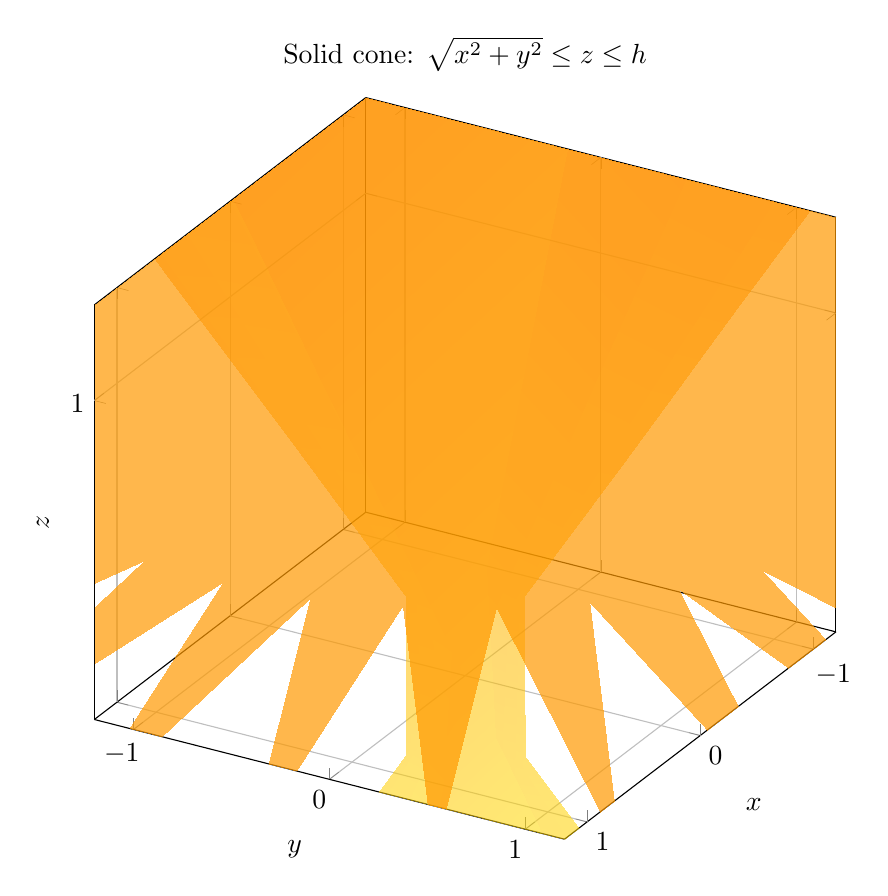
\begin{tikzpicture}
\begin{axis}[
    title={Solid cone: $\sqrt{x^2+y^2} \leq z \leq h$},
    xlabel=$x$, ylabel=$y$, zlabel=$z$,
    width=11cm, height=11cm,
    view={120}{30},
    xmin=-1.2, xmax=1.2, ymin=-1.2, ymax=1.2, zmin=0, zmax=1.3,
    xtick={-1,0,1}, ytick={-1,0,1}, ztick={1},
    grid=major,
    samples=20, samples y=20,
]
% Cone slanted side (parametric)
\addplot3[surf, shader=interp, opacity=0.55, draw=blue, fill=blue!30]
    ({(x)*cos(y*360)}, {(x)*sin(y*360)}, {x});
% Top disk
\addplot3[surf, shader=interp, opacity=0.7, draw=red, fill=red!50]
    ({x*cos(y*360)}, {x*sin(y*360)}, 1);
\end{axis}
\end{tikzpicture}
\end{document}
